\documentclass{article}
\usepackage{graphicx}
\usepackage{subcaption}
\usepackage{geometry}
\usepackage{hyperref}
\usepackage{grffile} % To handle dots and special characters in filenames

\geometry{
    a4paper,
    margin=0.6in
}

\hypersetup{
    colorlinks=true,
    linkcolor=blue,
    filecolor=magenta,      
    urlcolor=cyan,
}

\title{ALIE Byzantine Attack Comparison:\\Different Delta Values (CNN Simplest Sweep)}
\author{ByzFL SNN Benchmark}
\date{\today}

\begin{document}

\maketitle

\tableofcontents
\newpage

\section{Introduction}
This document presents comparison grids (2x2 subfigures) of the MNIST CNN model under the Optimal A Little Is Enough (ALIE) Byzantine attack. We compare four different step size ($\delta$) parameters:
\begin{itemize}
    \item \textbf{ALIE $\delta=10$} (Default positive large step size)
    \item \textbf{ALIE $\delta=1$} (Positive small step size)
    \item \textbf{ALIE $\delta=-1$} (Negative small step size)
    \item \textbf{ALIE $\delta=-10$} (Negative large step size)
\end{itemize}

Each comparison illustrates the test accuracy under varying numbers of Byzantine clients ($f \in [0, 2, 4, 5]$) and data heterogeneity levels ($\gamma \in [0.0, 0.33, 0.66, 1.0]$) with a total of $N = 10$ honest clients.

\newpage

\section{ALIE Attack: Best Aggregator Choice}
This section compares performance under ALIE using the dynamically selected best overall aggregator.

\begin{figure}[htbp]
    \centering
    \begin{subfigure}[b]{0.48\textwidth}
        \centering
        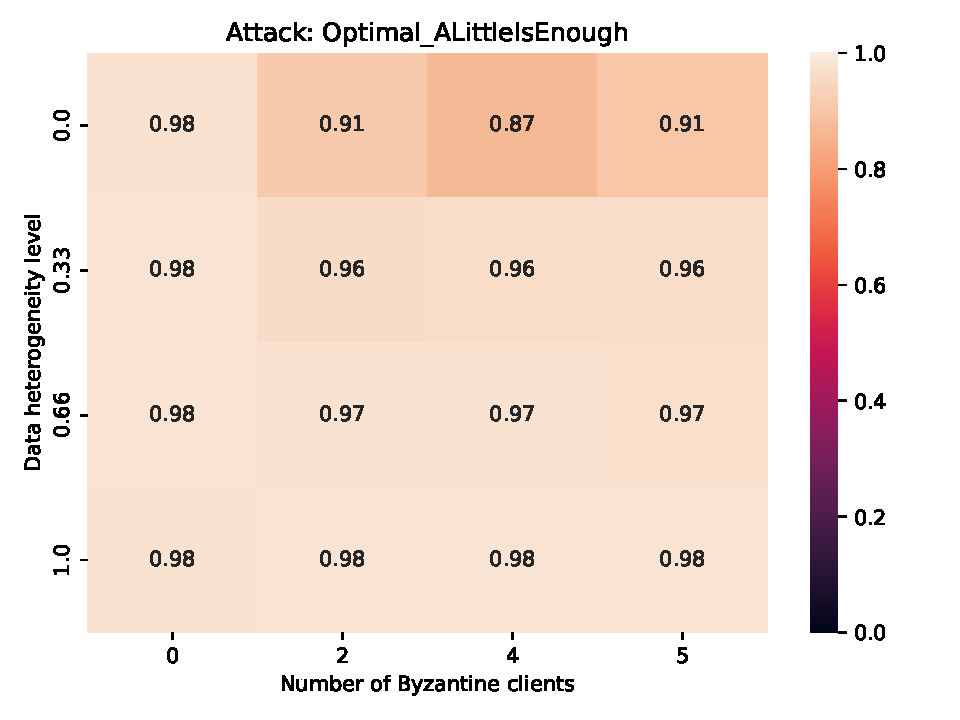
\includegraphics[width=\textwidth]{cnn_simplest_plots/best_test_Optimal_ALittleIsEnough_mnist_cnn_mnist_gamma_similarity_niid_NNM_ARC_nb_honest_clients_10_tolerated_f_equal_real.pdf}
        \caption{ALIE $\delta=10$}
        \label{fig:alie_10_best}
    \end{subfigure}
    \hfill
    \begin{subfigure}[b]{0.48\textwidth}
        \centering
        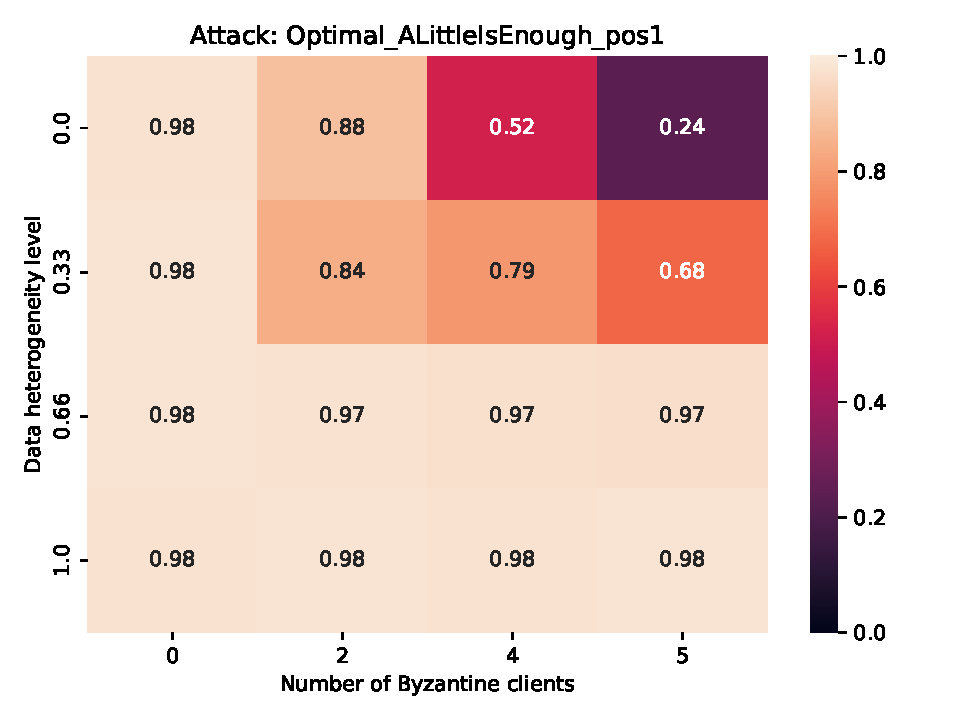
\includegraphics[width=\textwidth]{cnn_simplest_plots/best_test_Optimal_ALittleIsEnough_pos1_mnist_cnn_mnist_gamma_similarity_niid_NNM_ARC_nb_honest_clients_10_tolerated_f_equal_real.pdf}
        \caption{ALIE $\delta=1$}
        \label{fig:alie_pos1_best}
    \end{subfigure}
    
    \vspace{0.3cm}
    
    \begin{subfigure}[b]{0.48\textwidth}
        \centering
        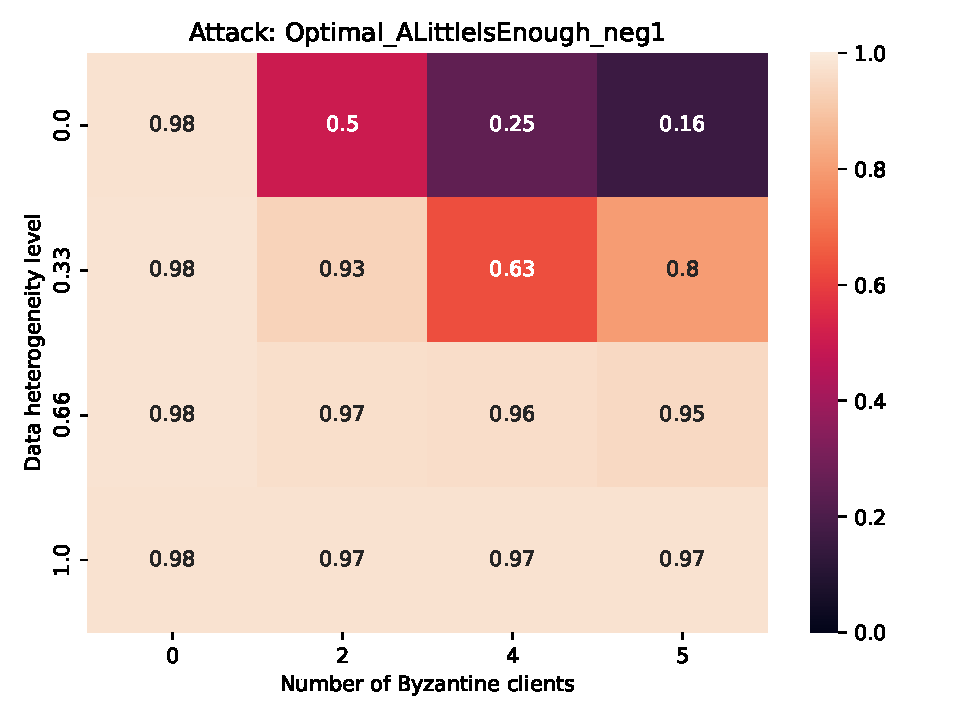
\includegraphics[width=\textwidth]{cnn_simplest_plots/best_test_Optimal_ALittleIsEnough_neg1_mnist_cnn_mnist_gamma_similarity_niid_NNM_ARC_nb_honest_clients_10_tolerated_f_equal_real.pdf}
        \caption{ALIE $\delta=-1$}
        \label{fig:alie_neg1_best}
    \end{subfigure}
    \hfill
    \begin{subfigure}[b]{0.48\textwidth}
        \centering
        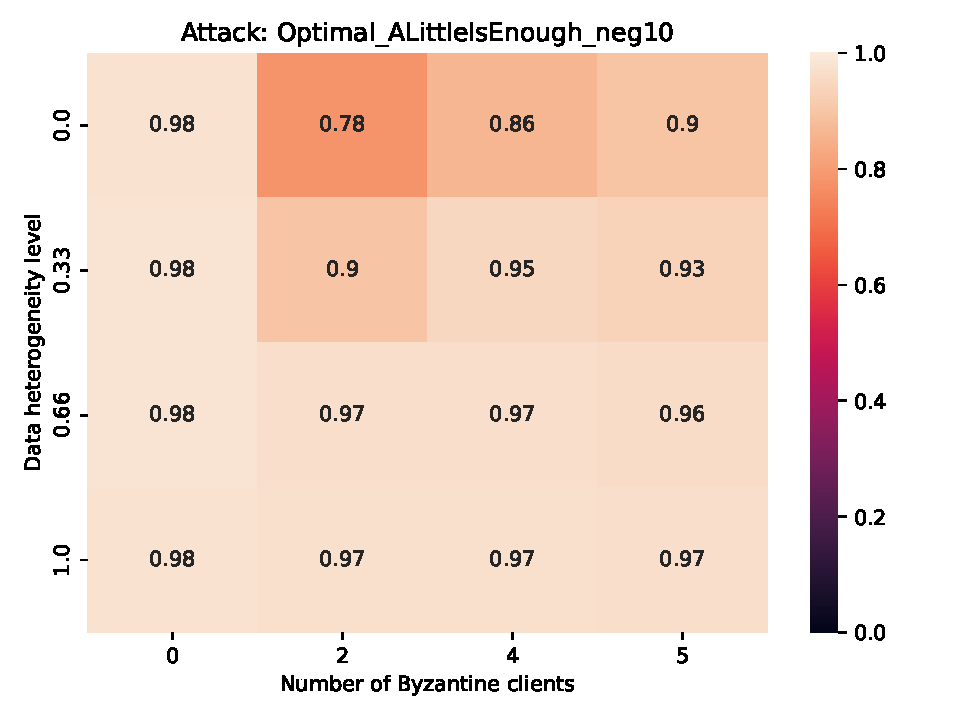
\includegraphics[width=\textwidth]{cnn_simplest_plots/best_test_Optimal_ALittleIsEnough_neg10_mnist_cnn_mnist_gamma_similarity_niid_NNM_ARC_nb_honest_clients_10_tolerated_f_equal_real.pdf}
        \caption{ALIE $\delta=-10$}
        \label{fig:alie_neg10_best}
    \end{subfigure}
    \caption{Accuracy comparison under ALIE attacks using the best overall aggregator selection.}
    \label{fig:best_overall}
\end{figure}

\clearpage

\section{ALIE Attack: Centered Clipping}
This section compares performance under ALIE using Centered Clipping.

\begin{figure}[htbp]
    \centering
    \begin{subfigure}[b]{0.48\textwidth}
        \centering
        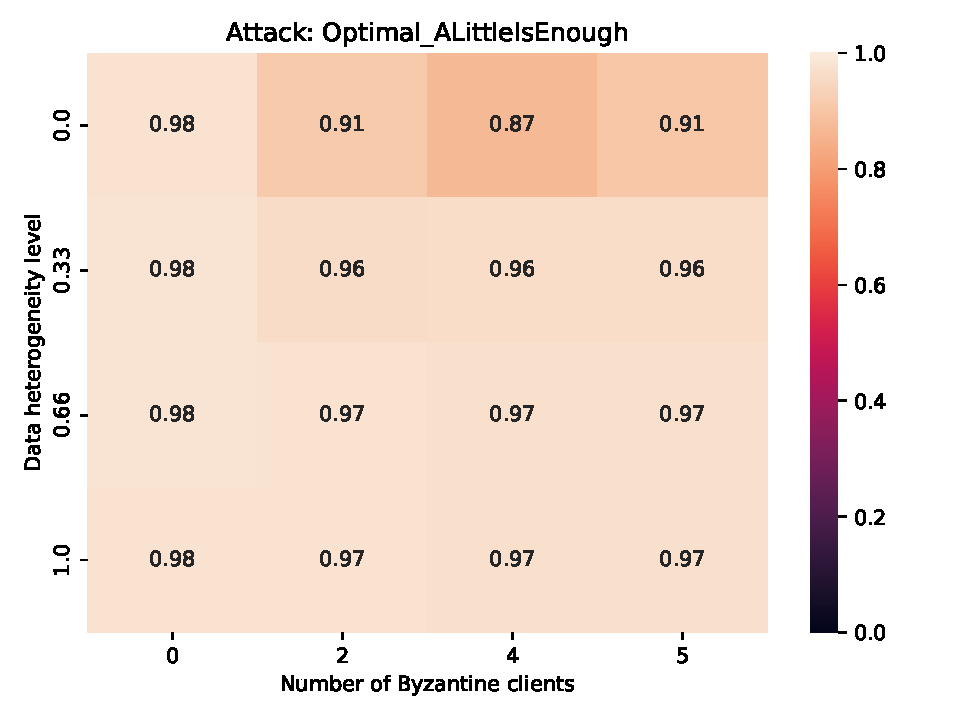
\includegraphics[width=\textwidth]{cnn_simplest_plots/test_Optimal_ALittleIsEnough_mnist_cnn_mnist_gamma_similarity_niid_NNM_ARC_CenteredClipping_nb_honest_clients_10_tolerated_f_equal_real.pdf}
        \caption{ALIE $\delta=10$}
        \label{fig:alie_10_cc}
    \end{subfigure}
    \hfill
    \begin{subfigure}[b]{0.48\textwidth}
        \centering
        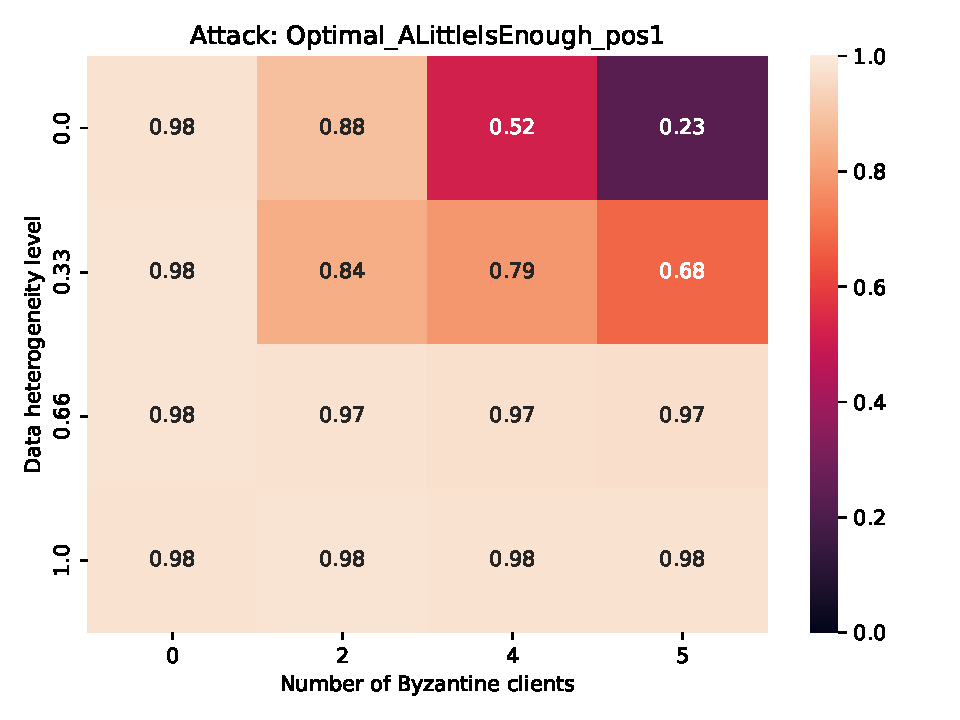
\includegraphics[width=\textwidth]{cnn_simplest_plots/test_Optimal_ALittleIsEnough_pos1_mnist_cnn_mnist_gamma_similarity_niid_NNM_ARC_CenteredClipping_nb_honest_clients_10_tolerated_f_equal_real.pdf}
        \caption{ALIE $\delta=1$}
        \label{fig:alie_pos1_cc}
    \end{subfigure}
    
    \vspace{0.3cm}
    
    \begin{subfigure}[b]{0.48\textwidth}
        \centering
        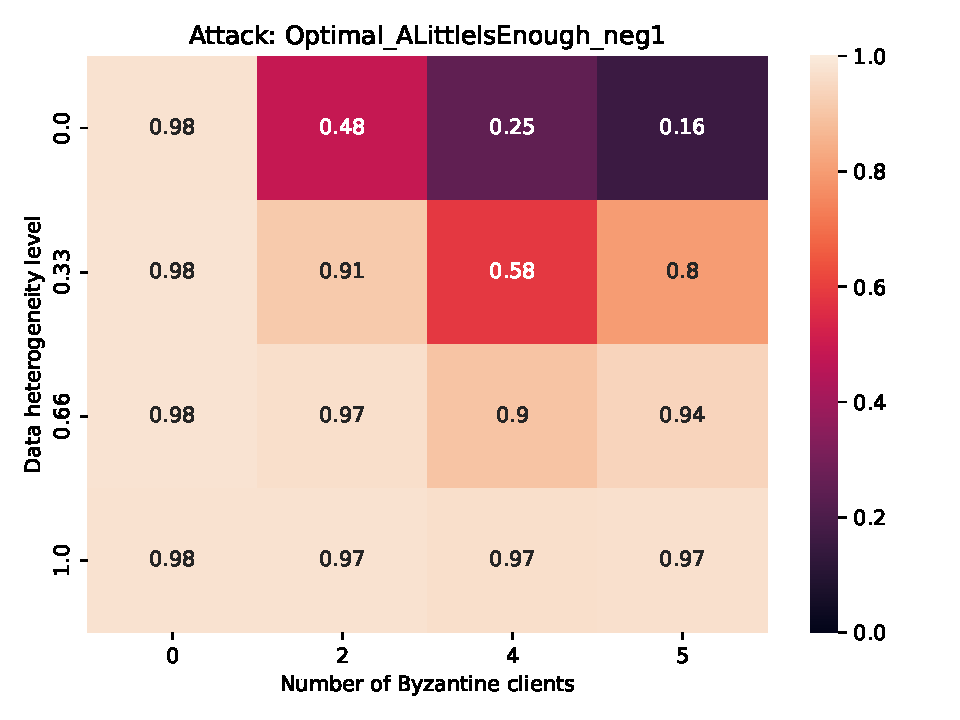
\includegraphics[width=\textwidth]{cnn_simplest_plots/test_Optimal_ALittleIsEnough_neg1_mnist_cnn_mnist_gamma_similarity_niid_NNM_ARC_CenteredClipping_nb_honest_clients_10_tolerated_f_equal_real.pdf}
        \caption{ALIE $\delta=-1$}
        \label{fig:alie_neg1_cc}
    \end{subfigure}
    \hfill
    \begin{subfigure}[b]{0.48\textwidth}
        \centering
        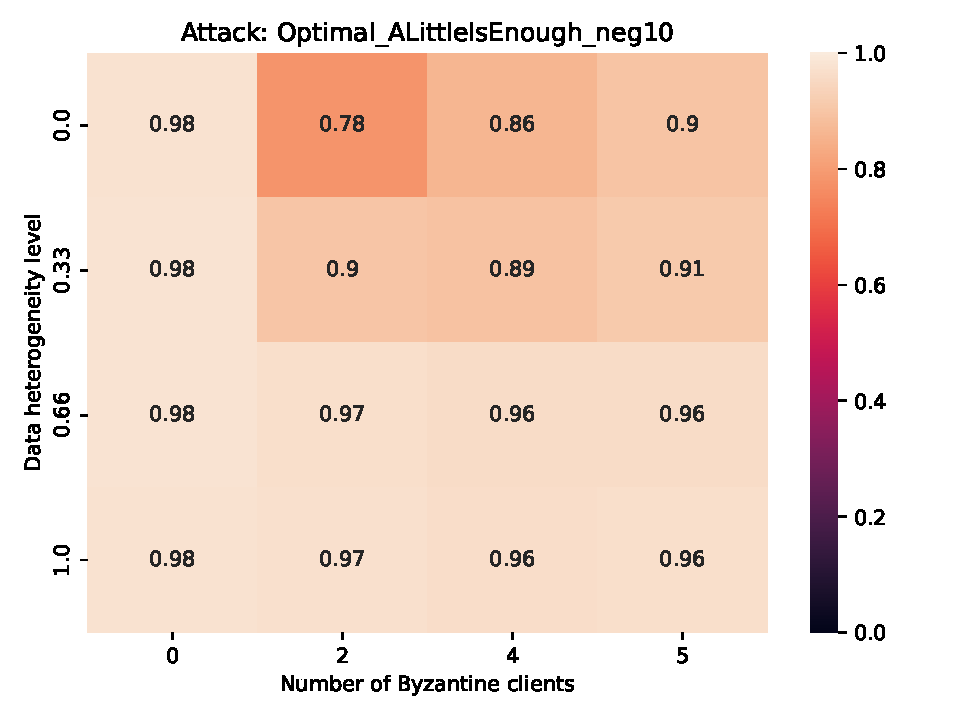
\includegraphics[width=\textwidth]{cnn_simplest_plots/test_Optimal_ALittleIsEnough_neg10_mnist_cnn_mnist_gamma_similarity_niid_NNM_ARC_CenteredClipping_nb_honest_clients_10_tolerated_f_equal_real.pdf}
        \caption{ALIE $\delta=-10$}
        \label{fig:alie_neg10_cc}
    \end{subfigure}
    \caption{Accuracy comparison under ALIE attacks using Centered Clipping.}
    \label{fig:cc_comparison}
\end{figure}

\clearpage

\section{ALIE Attack: Geometric Median}
This section compares performance under ALIE using Geometric Median.

\begin{figure}[htbp]
    \centering
    \begin{subfigure}[b]{0.48\textwidth}
        \centering
        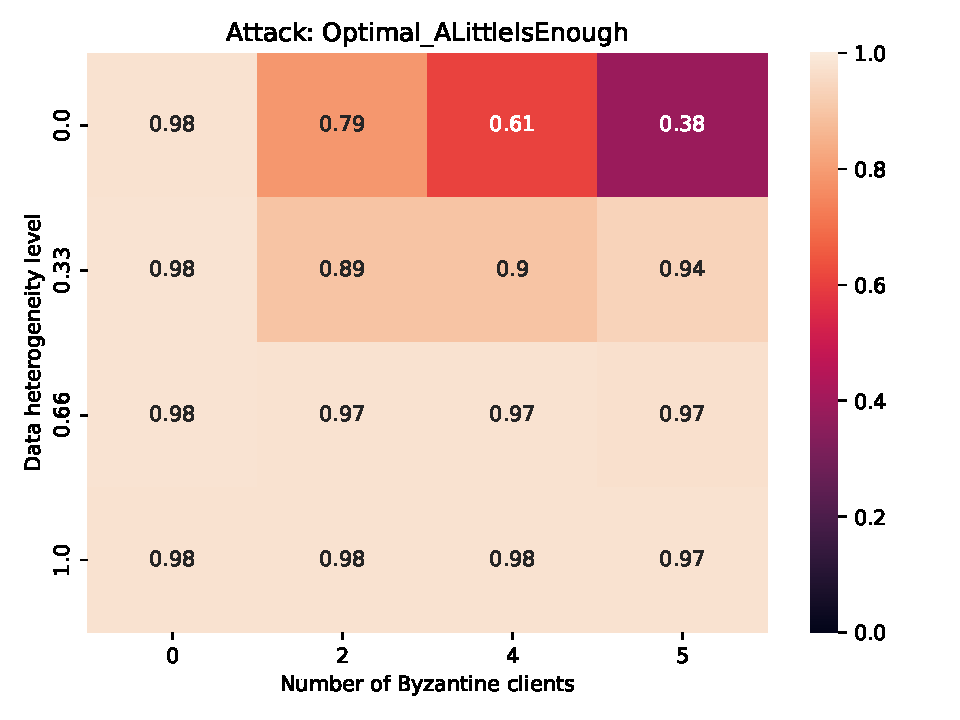
\includegraphics[width=\textwidth]{cnn_simplest_plots/test_Optimal_ALittleIsEnough_mnist_cnn_mnist_gamma_similarity_niid_NNM_ARC_GeometricMedian_nb_honest_clients_10_tolerated_f_equal_real.pdf}
        \caption{ALIE $\delta=10$}
        \label{fig:alie_10_gm}
    \end{subfigure}
    \hfill
    \begin{subfigure}[b]{0.48\textwidth}
        \centering
        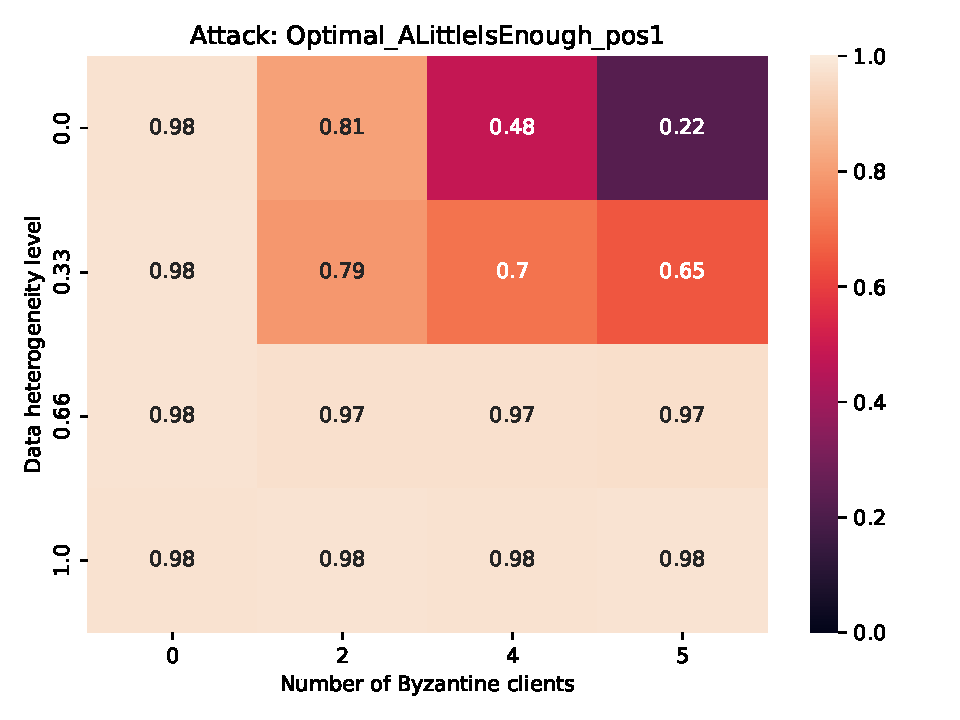
\includegraphics[width=\textwidth]{cnn_simplest_plots/test_Optimal_ALittleIsEnough_pos1_mnist_cnn_mnist_gamma_similarity_niid_NNM_ARC_GeometricMedian_nb_honest_clients_10_tolerated_f_equal_real.pdf}
        \caption{ALIE $\delta=1$}
        \label{fig:alie_pos1_gm}
    \end{subfigure}
    
    \vspace{0.3cm}
    
    \begin{subfigure}[b]{0.48\textwidth}
        \centering
        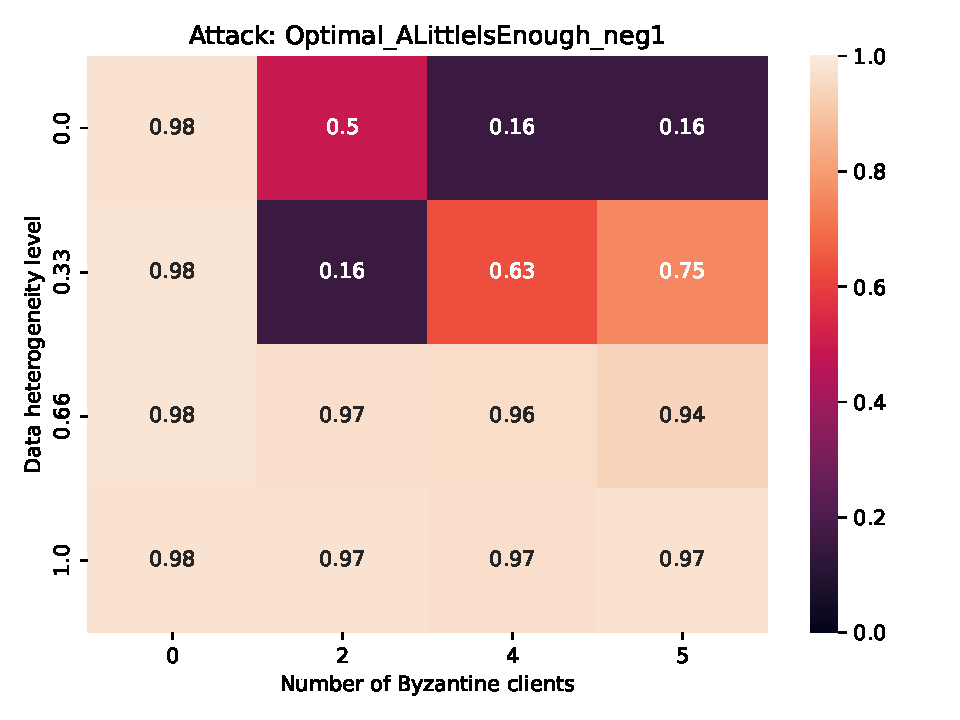
\includegraphics[width=\textwidth]{cnn_simplest_plots/test_Optimal_ALittleIsEnough_neg1_mnist_cnn_mnist_gamma_similarity_niid_NNM_ARC_GeometricMedian_nb_honest_clients_10_tolerated_f_equal_real.pdf}
        \caption{ALIE $\delta=-1$}
        \label{fig:alie_neg1_gm}
    \end{subfigure}
    \hfill
    \begin{subfigure}[b]{0.48\textwidth}
        \centering
        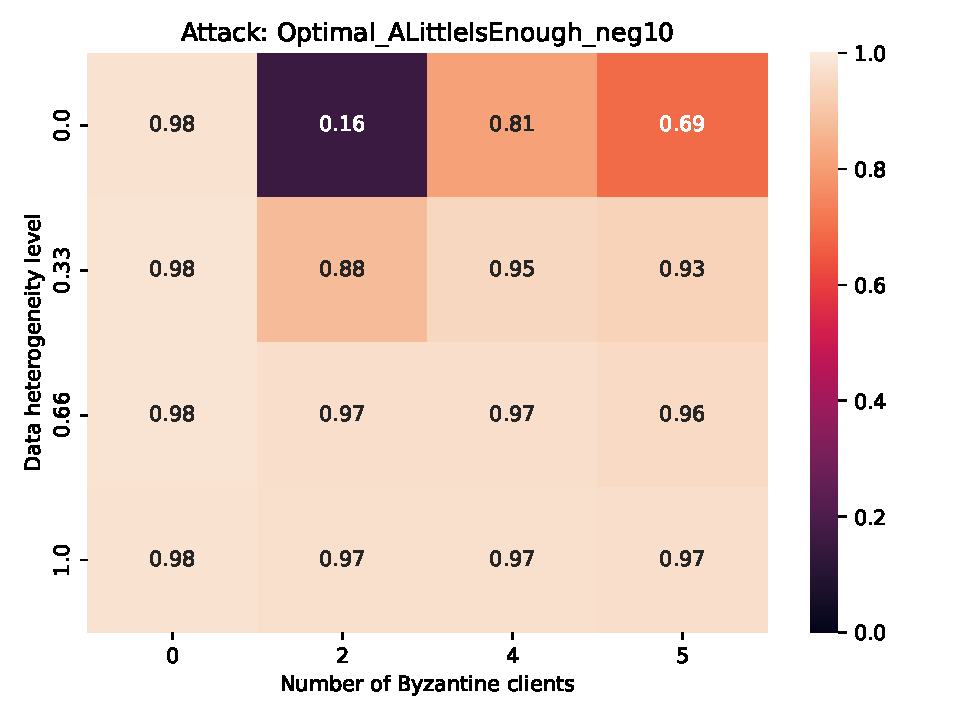
\includegraphics[width=\textwidth]{cnn_simplest_plots/test_Optimal_ALittleIsEnough_neg10_mnist_cnn_mnist_gamma_similarity_niid_NNM_ARC_GeometricMedian_nb_honest_clients_10_tolerated_f_equal_real.pdf}
        \caption{ALIE $\delta=-10$}
        \label{fig:alie_neg10_gm}
    \end{subfigure}
    \caption{Accuracy comparison under ALIE attacks using Geometric Median.}
    \label{fig:gm_comparison}
\end{figure}

\clearpage

\section{ALIE Attack: Multi-Krum}
This section compares performance under ALIE using Multi-Krum.

\begin{figure}[htbp]
    \centering
    \begin{subfigure}[b]{0.48\textwidth}
        \centering
        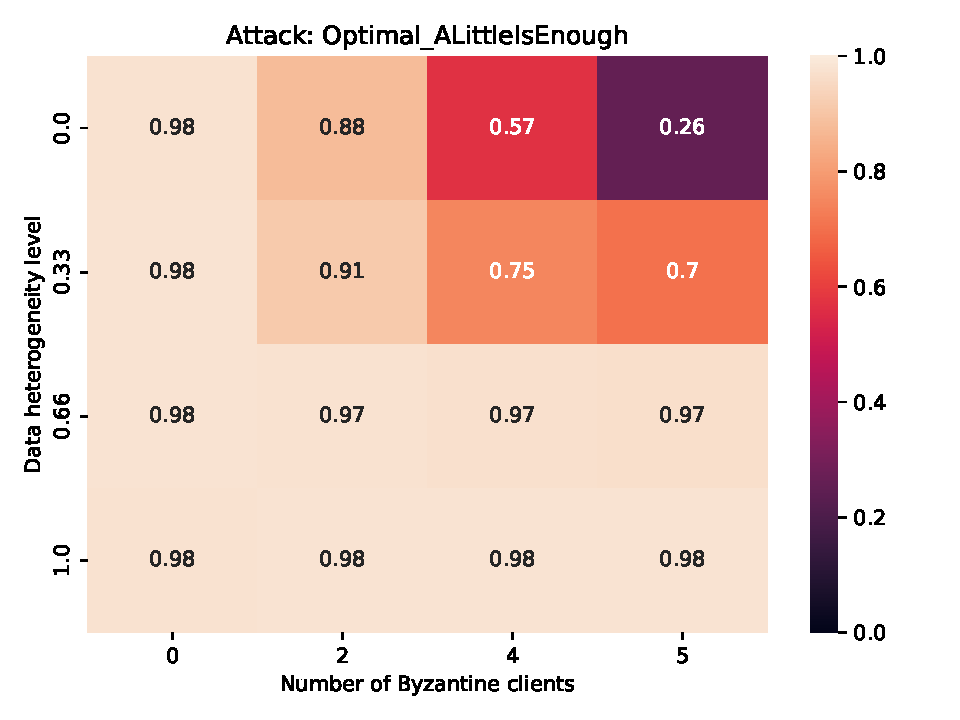
\includegraphics[width=\textwidth]{cnn_simplest_plots/test_Optimal_ALittleIsEnough_mnist_cnn_mnist_gamma_similarity_niid_NNM_ARC_MultiKrum_nb_honest_clients_10_tolerated_f_equal_real.pdf}
        \caption{ALIE $\delta=10$}
        \label{fig:alie_10_mk}
    \end{subfigure}
    \hfill
    \begin{subfigure}[b]{0.48\textwidth}
        \centering
        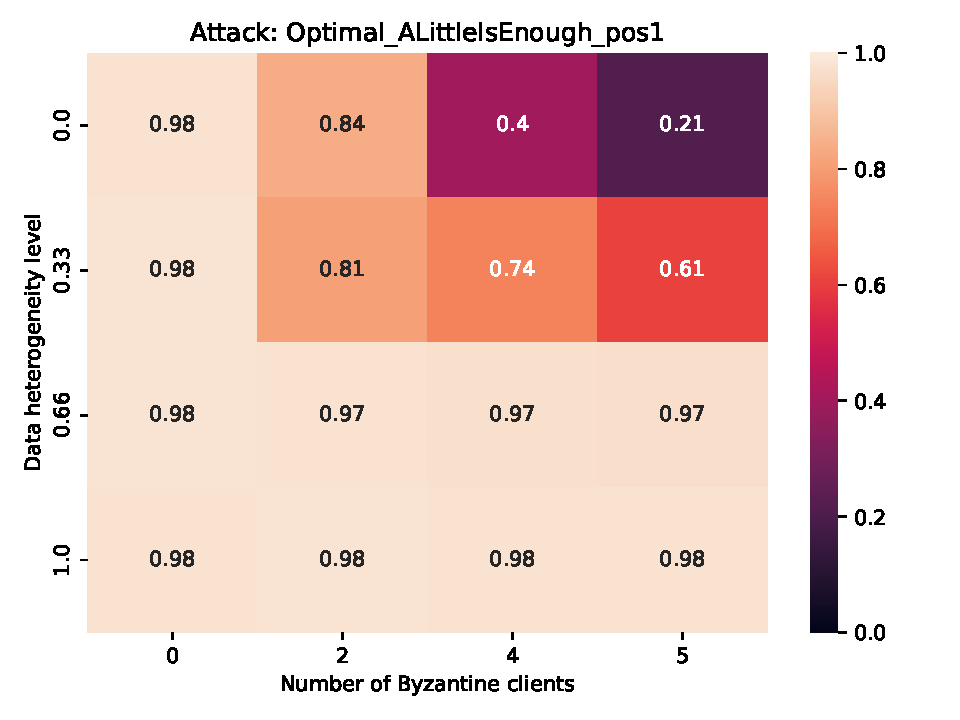
\includegraphics[width=\textwidth]{cnn_simplest_plots/test_Optimal_ALittleIsEnough_pos1_mnist_cnn_mnist_gamma_similarity_niid_NNM_ARC_MultiKrum_nb_honest_clients_10_tolerated_f_equal_real.pdf}
        \caption{ALIE $\delta=1$}
        \label{fig:alie_pos1_mk}
    \end{subfigure}
    
    \vspace{0.3cm}
    
    \begin{subfigure}[b]{0.48\textwidth}
        \centering
        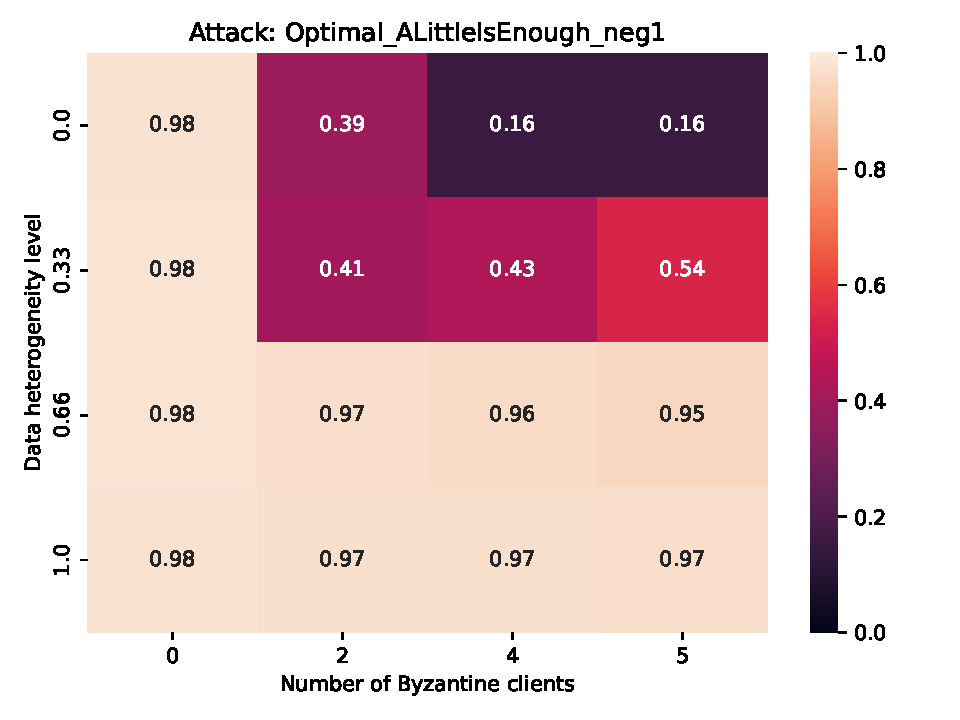
\includegraphics[width=\textwidth]{cnn_simplest_plots/test_Optimal_ALittleIsEnough_neg1_mnist_cnn_mnist_gamma_similarity_niid_NNM_ARC_MultiKrum_nb_honest_clients_10_tolerated_f_equal_real.pdf}
        \caption{ALIE $\delta=-1$}
        \label{fig:alie_neg1_mk}
    \end{subfigure}
    \hfill
    \begin{subfigure}[b]{0.48\textwidth}
        \centering
        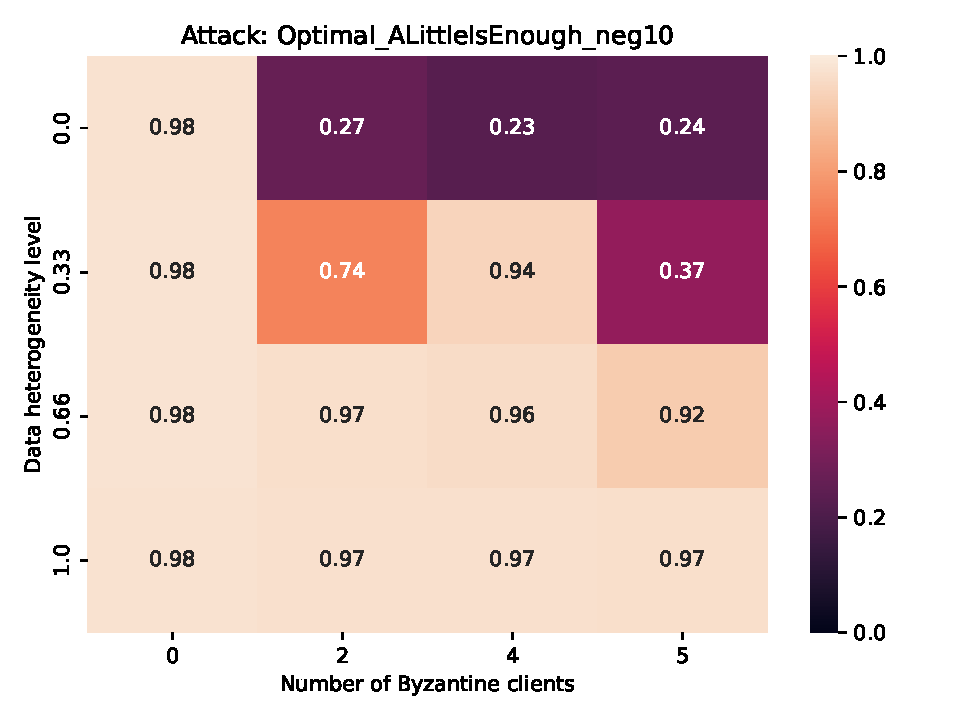
\includegraphics[width=\textwidth]{cnn_simplest_plots/test_Optimal_ALittleIsEnough_neg10_mnist_cnn_mnist_gamma_similarity_niid_NNM_ARC_MultiKrum_nb_honest_clients_10_tolerated_f_equal_real.pdf}
        \caption{ALIE $\delta=-10$}
        \label{fig:alie_neg10_mk}
    \end{subfigure}
    \caption{Accuracy comparison under ALIE attacks using Multi-Krum.}
    \label{fig:mk_comparison}
\end{figure}

\clearpage

\section{ALIE Attack: Trimmed Mean}
This section compares performance under ALIE using Trimmed Mean.

\begin{figure}[htbp]
    \centering
    \begin{subfigure}[b]{0.48\textwidth}
        \centering
        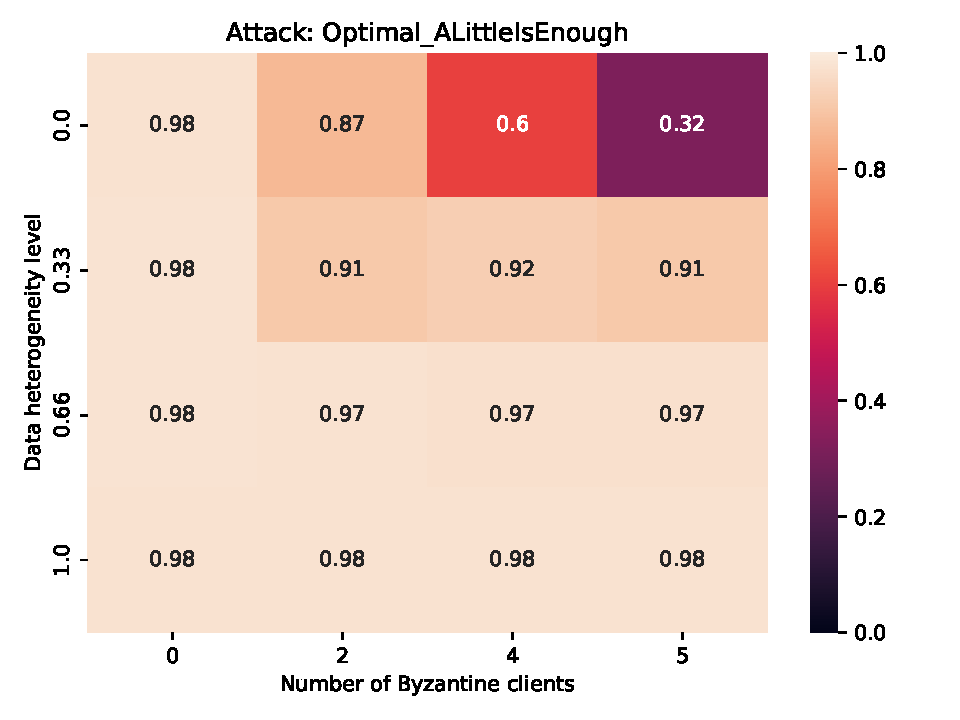
\includegraphics[width=\textwidth]{cnn_simplest_plots/test_Optimal_ALittleIsEnough_mnist_cnn_mnist_gamma_similarity_niid_NNM_ARC_TrMean_nb_honest_clients_10_tolerated_f_equal_real.pdf}
        \caption{ALIE $\delta=10$}
        \label{fig:alie_10_tm}
    \end{subfigure}
    \hfill
    \begin{subfigure}[b]{0.48\textwidth}
        \centering
        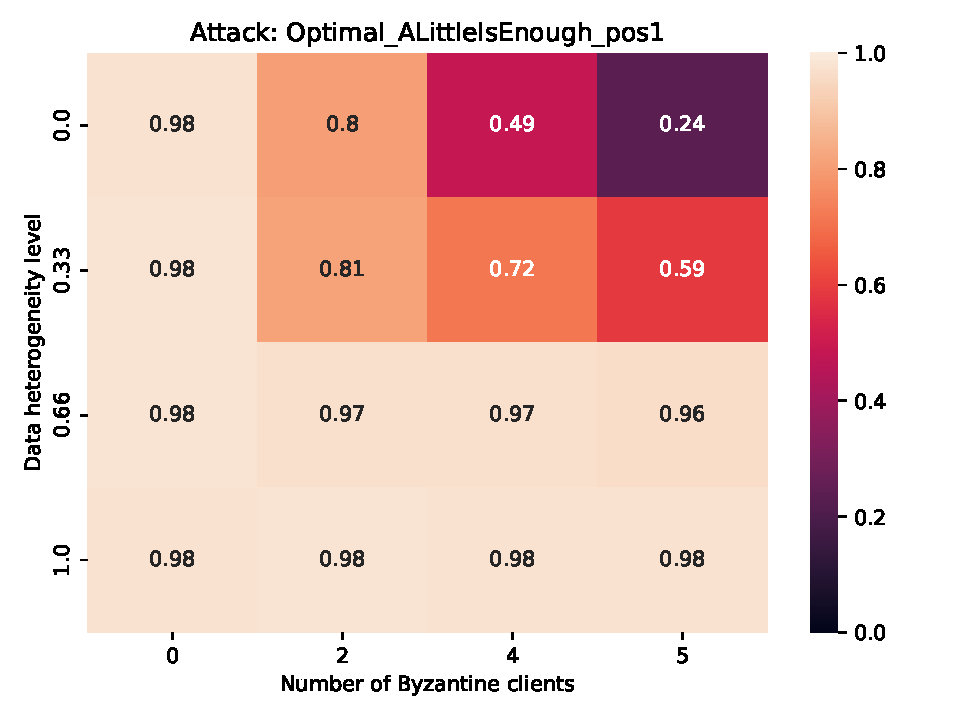
\includegraphics[width=\textwidth]{cnn_simplest_plots/test_Optimal_ALittleIsEnough_pos1_mnist_cnn_mnist_gamma_similarity_niid_NNM_ARC_TrMean_nb_honest_clients_10_tolerated_f_equal_real.pdf}
        \caption{ALIE $\delta=1$}
        \label{fig:alie_pos1_tm}
    \end{subfigure}
    
    \vspace{0.3cm}
    
    \begin{subfigure}[b]{0.48\textwidth}
        \centering
        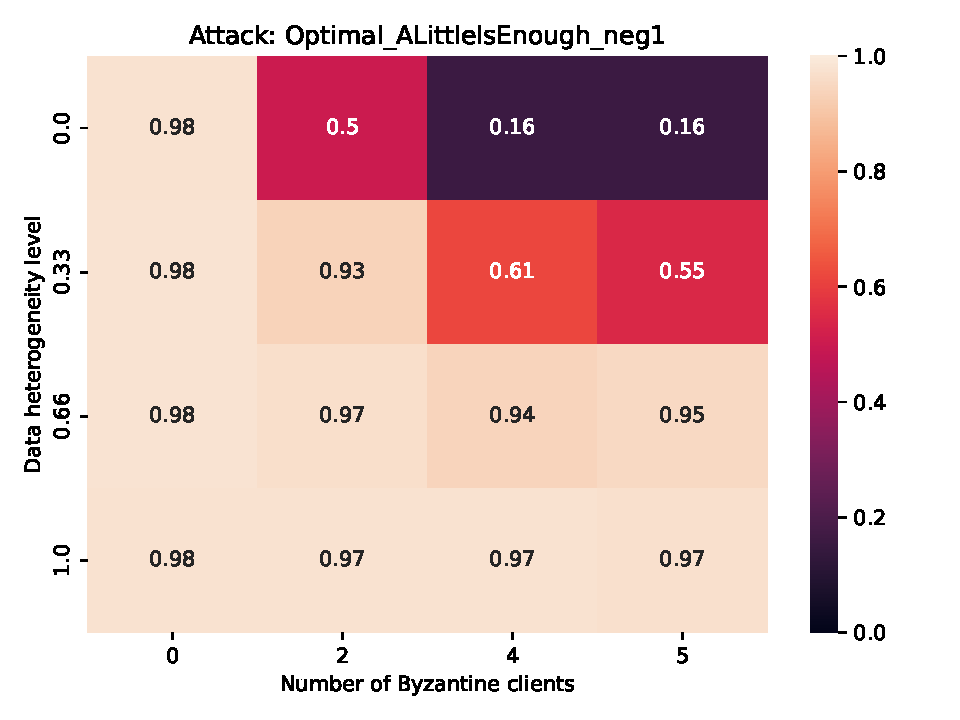
\includegraphics[width=\textwidth]{cnn_simplest_plots/test_Optimal_ALittleIsEnough_neg1_mnist_cnn_mnist_gamma_similarity_niid_NNM_ARC_TrMean_nb_honest_clients_10_tolerated_f_equal_real.pdf}
        \caption{ALIE $\delta=-1$}
        \label{fig:alie_neg1_tm}
    \end{subfigure}
    \hfill
    \begin{subfigure}[b]{0.48\textwidth}
        \centering
        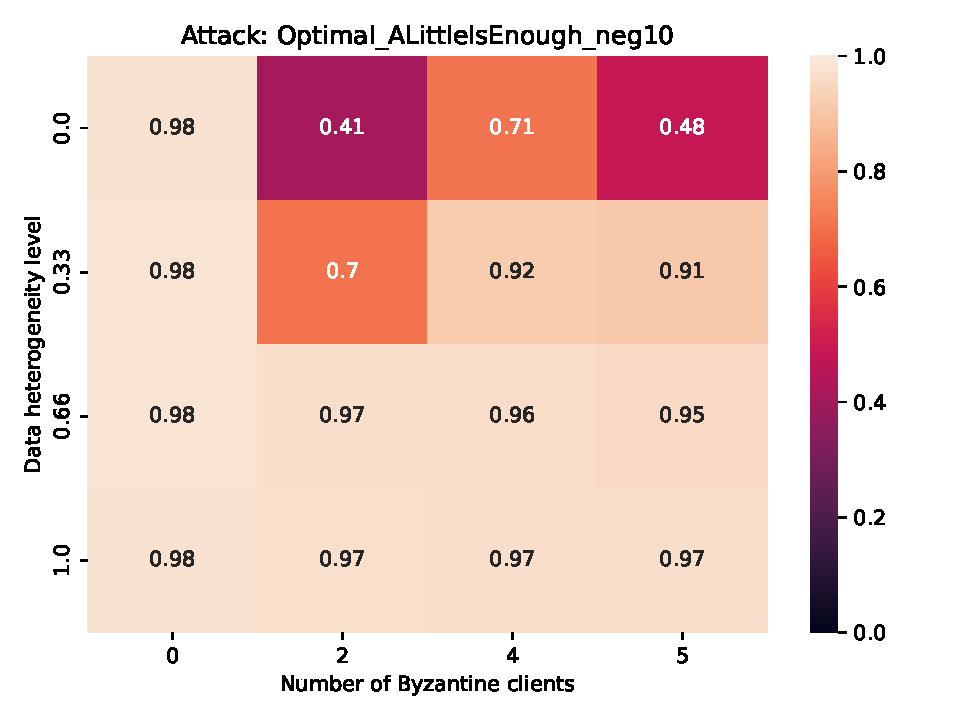
\includegraphics[width=\textwidth]{cnn_simplest_plots/test_Optimal_ALittleIsEnough_neg10_mnist_cnn_mnist_gamma_similarity_niid_NNM_ARC_TrMean_nb_honest_clients_10_tolerated_f_equal_real.pdf}
        \caption{ALIE $\delta=-10$}
        \label{fig:alie_neg10_tm}
    \end{subfigure}
    \caption{Accuracy comparison under ALIE attacks using Trimmed Mean.}
    \label{fig:tm_comparison}
\end{figure}

\end{document}
